\section{Question 1}
\subsection{Circuit diagram}
\begin{figure}[H]
    \centering
    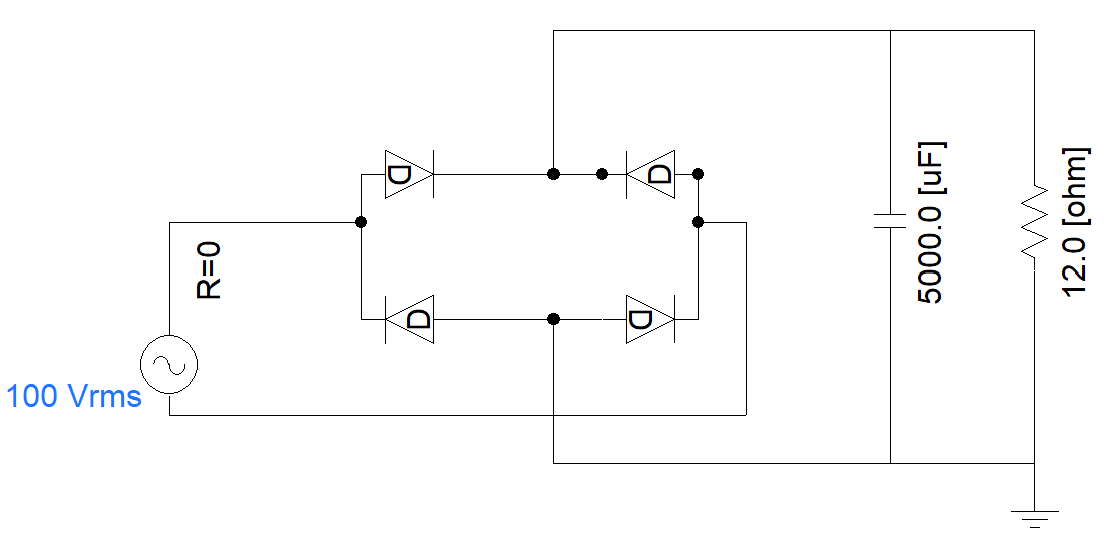
\includegraphics[width = \textwidth]{img/figure1.png}
    \caption{Circuit diagram for question 1.}
\end{figure}
\subsection{Instantaneous voltages}
\begin{figure}[H]
    \centering
    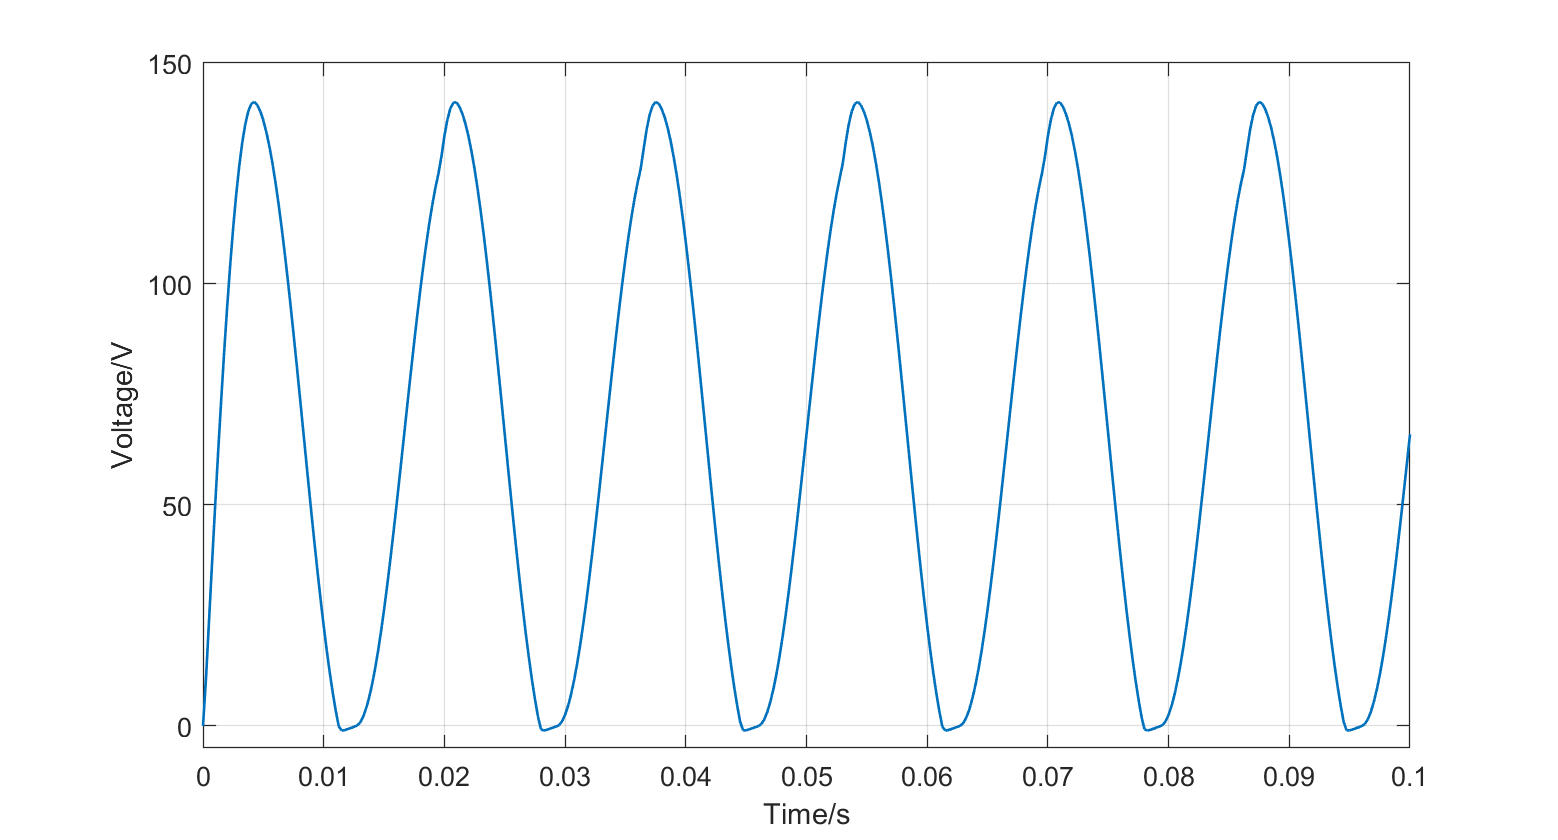
\includegraphics[width = \textwidth]{img/figure2.png}
    \caption{Graph to show instantaneous input voltage across the voltage source.}
\end{figure}
\begin{figure}[H]
    \centering
    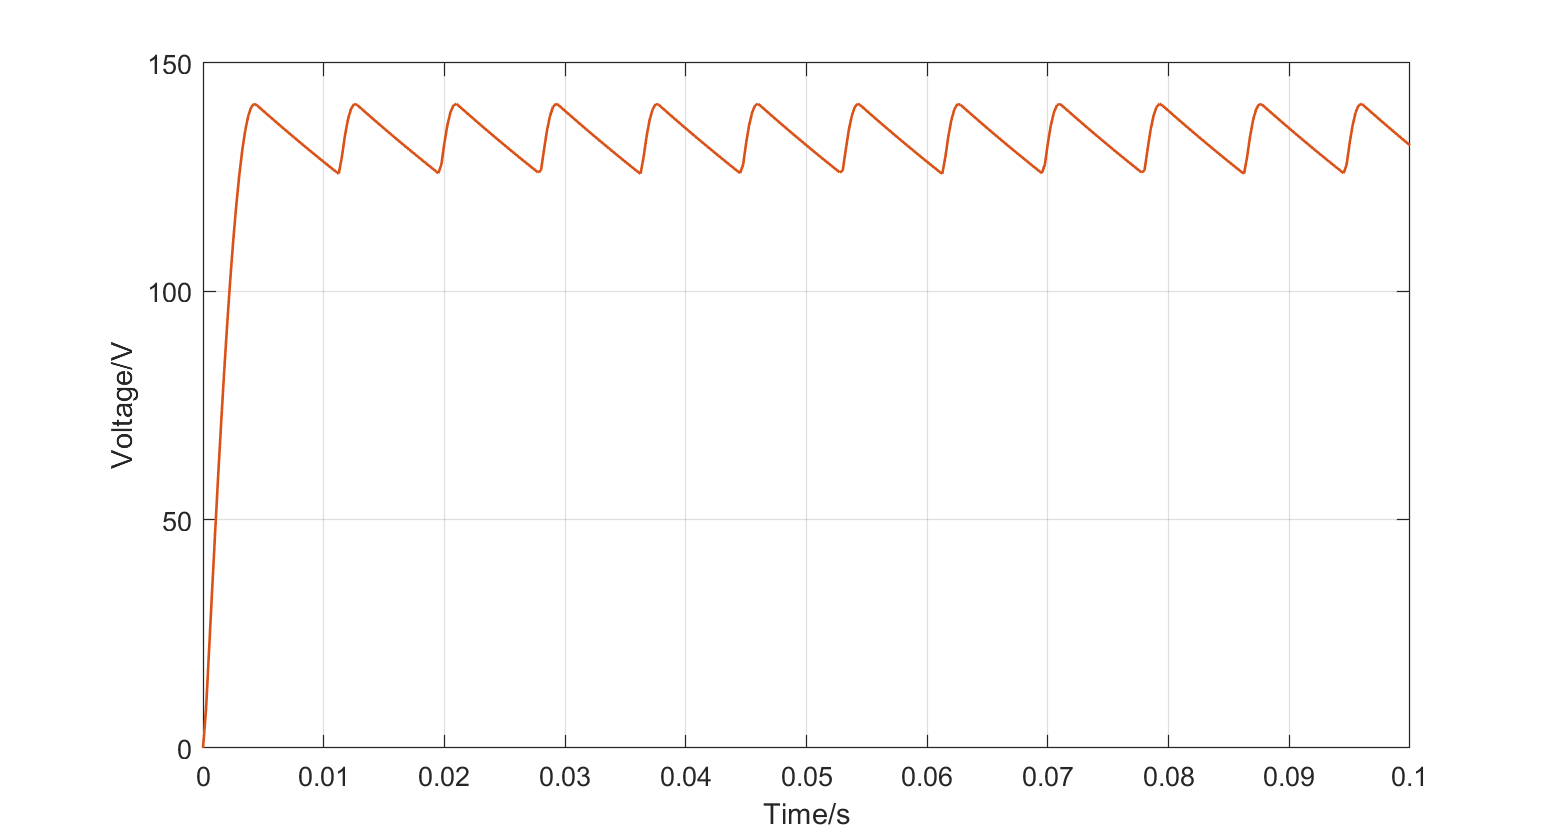
\includegraphics[width = \textwidth]{img/figure3.png}
    \caption{Graph to show instantaneous output voltage across the resistive load.}
    \label{fig:resistiveLoad}
\end{figure}
\subsection{Effect of increasing capacitcance to \SI{25}{\micro\farad}}
\begin{figure}[H]
    \centering
    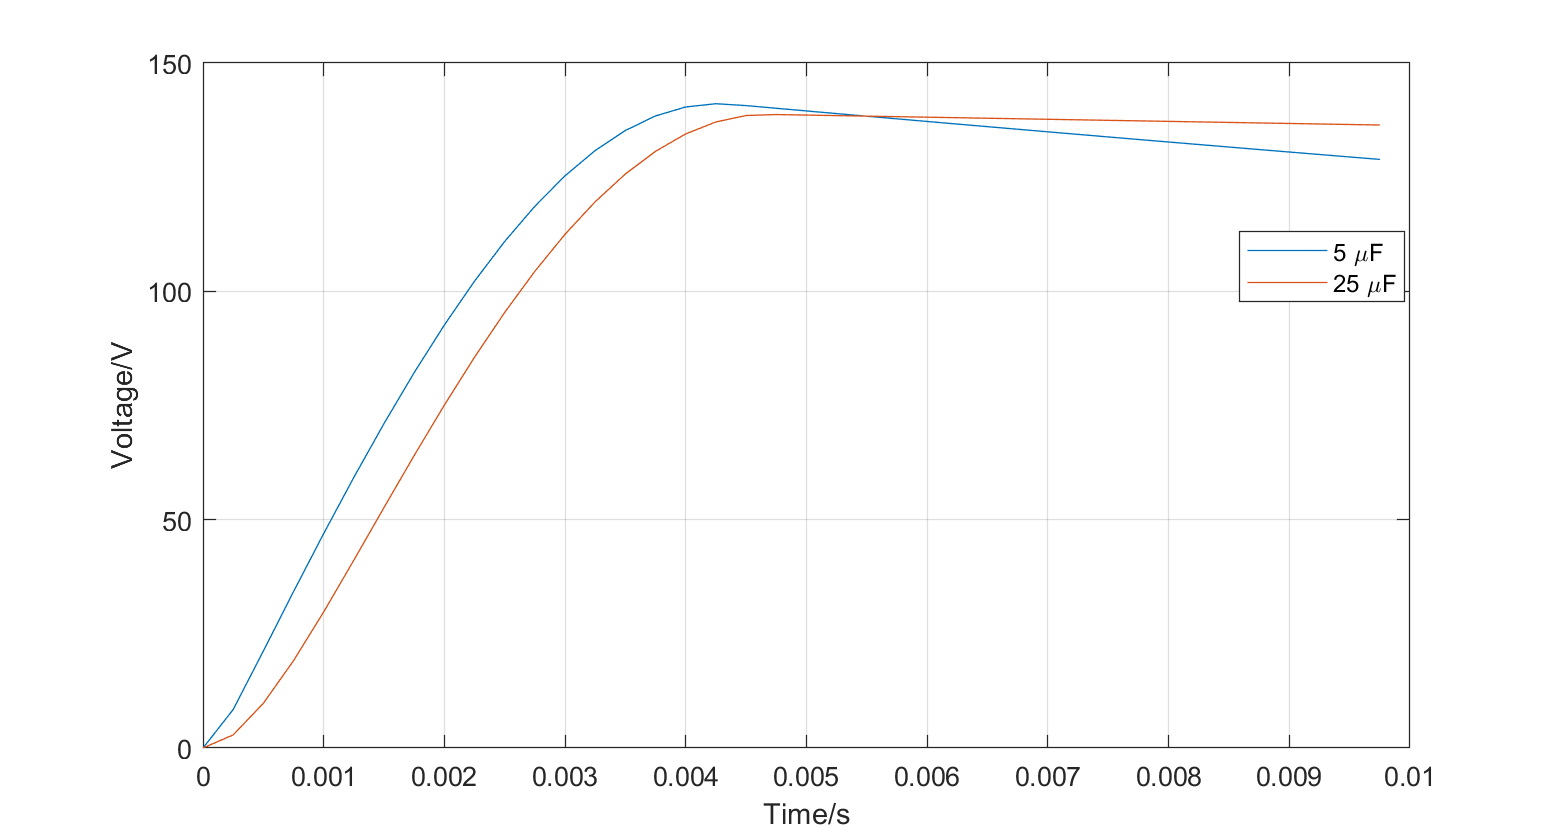
\includegraphics[width = \textwidth]{img/figure4.png}
    \caption{Graph to show comparison between instantaneous output voltage across the resistive load for different capacitance values.}
    \label{fig:comp1}
\end{figure}
The purpose of the capacitor in this diode bridge circuit is to filter/reduce the amount of voltage ripple, inherent to bridge diode circuits. We can see in Figure \ref{fig:resistiveLoad} that our voltage drop is approximately \SI{25}{\volt} between pulses. By increasing the capacitance, our voltage drop reduces (from data: voltage drop with \SI{25}{\micro\farad} $\approx \SI{4}{\volt}$.) This is desirable as this achieves a more stable DC output. However, increasing the capacitance also increases the rise time and reduces the peak voltage of the output, shown in Figure \ref{fig:comp1}.